\chapter{Reinforcement Learning for Adaptive Sliding-Velocity Optimization}
\label{chap:rl}
\section{Motivation}
A full-coverage path guarantees that the tool footprint visits the target surface, but it does not guarantee uniform material removal. Contact force varies with curvature, fixture error, pad deformation, sensor bias, and admittance dynamics. Under a constant feed speed, these force variations produce non-uniform pressure--velocity products and therefore non-uniform removal.

\begin{figure}[t]
    \centering
    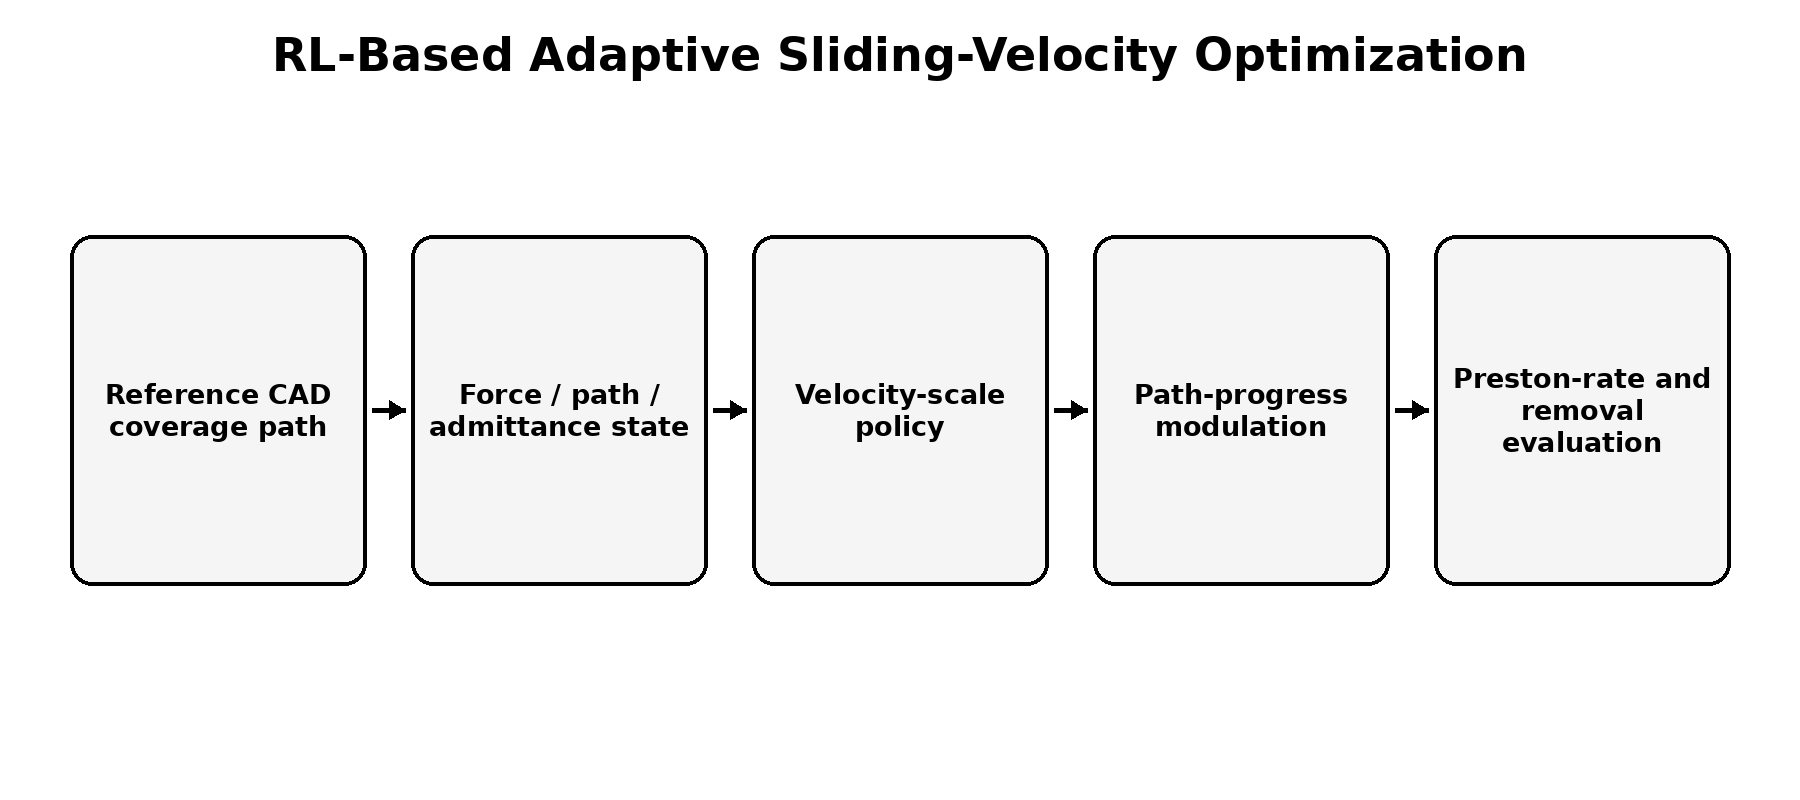
\includegraphics[width=0.98\textwidth]{./4.ReinforcementLearning/figs/rl_velocity_pipeline.png}
    \caption{Hierarchical RL formulation. The policy changes only the path-progress rate while preserving the CAD path and the low-level admittance controller.}
    \label{fig:rl_pipeline}
\end{figure}

\section{Restricted RL Formulation}
The policy does not generate robot joint commands or a new Cartesian pose. At time $t$, the observation is
\begin{equation}
\mathbf{o}_t^{\mathrm{RL}}=[F_{n,t},\mathbf{F}_{t-h:t},F_n^*,\dot{s}_t,\kappa_t,\phi_t,\mathbf{x}_{a,t}],
\end{equation}
where $F_{n,t}$ is the measured normal force, $\mathbf{F}_{t-h:t}$ is a wrench history, $F_n^*$ is the desired force, $\dot{s}_t$ is current path progress, $\kappa_t$ is local curvature, $\phi_t$ is the normalized path phase, and $\mathbf{x}_{a,t}$ contains admittance states.

The action is a bounded velocity scale
\begin{equation}
\alpha_t \in [\alpha_{\min},\alpha_{\max}], \qquad \dot{s}_{t+1}=\alpha_t\dot{s}_{\mathrm{nom}}.
\end{equation}
Action-rate limits and low-pass filtering prevent chatter.

\section{Preston-Based Reward}
The local material-removal rate is approximated by
\begin{equation}
\rho_t = K p_t v_t,
\end{equation}
where $p_t$ is estimated from normal force and contact area and $v_t$ is the sliding velocity. The policy tracks a target rate $\rho^*$:
\begin{equation}
r_t = -w_{\rho}(\rho_t-\rho^*)^2 - w_{\alpha}(\Delta\alpha_t)^2 - w_J J_t^2 - w_S P_{\mathrm{safety}}.
\end{equation}
The smoothness term penalizes rapid velocity changes, and $P_{\mathrm{safety}}$ penalizes overload, contact loss, excessive tracking error, or unsafe tool motion.

\section{Training Environment}
Training is performed in a parallel simulation environment using the same reference paths used by the real controller. Domain randomization covers curvature, friction, pad stiffness, force-sensor bias, delay, noise, initial pose error, and contact parameters. The policy can be trained using PPO or another actor--critic method, although the exact algorithm is secondary to the restricted hierarchical formulation.

\section{Analytical and Model-Based Baselines}
A strong inverse-Preston controller is
\begin{equation}
v_t = \mathrm{clip}\left(\frac{c}{p_t+\epsilon},v_{\min},v_{\max}\right).
\end{equation}
A filtered PID or model-predictive speed controller can regulate $\rho_t-\rho^*$. These baselines are essential. RL is justified only if it provides better robustness under delay, saturation, curvature transitions, contact-area uncertainty, and noisy force estimates. If the analytical controller performs equivalently, RL adds unnecessary complexity.

\section{Internal Preliminary Results}
Internal simulation work has shown that adaptive velocity can strongly reduce Preston-rate variation. On a flat surface, the coefficient of variation decreased from 0.101 under fixed velocity to 0.013 under the learned policy. On a convex surface, the value decreased from 0.195 to 0.026. These results are preliminary and should not be interpreted as measured material-removal performance. Real-robot experiments and direct removal measurements are required.

\section{Sim-to-Real Transfer and Safety}
The real system uses the same observation normalization, action limits, and path-phase representation as simulation. Safety overrides the learned scale when force or path error exceeds a threshold. A gradual deployment sequence is used: offline replay, zero-contact motion, compliant contact on sacrificial coupons, and finally workpiece experiments. The learned policy is never allowed to modify the geometric path or exceed the certified speed and force envelope.
